\documentclass[10pt,letterpaper,twoside]{article}
\usepackage{code/manuscript_assets/researchpreprint}
\usepackage[T1]{fontenc}
\usepackage{amsmath,amssymb,amsthm,mathtools,bm}
\usepackage{booktabs,array}
\usepackage{graphicx}
\usepackage{microtype}
\usepackage{url}
\usepackage{hyperref}
\hypersetup{hidelinks}
\setlength{\emergencystretch}{3em}

\newtheorem{theorem}{Theorem}
\newcommand{\R}{\mathbb{R}}
\newcommand{\norm}[1]{\left\lVert #1\right\rVert}
\newcommand{\AuditRecords}{144}
\newcommand{\AuditSources}{6}
\newcommand{\FeatureClasses}{32}
\newcommand{\LegacyFeatureCollisions}{60}
\newcommand{\LegacyTestRecords}{64}
\newcommand{\LegacyRawDuplicates}{18}
\newcommand{\LegacyRCOLMSE}{2.638e-04}
\newcommand{\LegacyKNNMSE}{3.644e-04}
\newcommand{\SourceKNNMSE}{2.052e-04}
\newcommand{\SourceHRegret}{3.193}
\newcommand{\SourceKNNRegret}{0.181}
\newcommand{\GroupedKNNMSE}{2.441e-03}
\newcommand{\GroupedHMSE}{2.526e-03}
\newcommand{\GroupedKNNRegret}{1.605}
\newcommand{\GroupedHRegret}{1.571}
\newcommand{\GroupedAffineRegret}{0.774}


\begin{document}

\title{Feature-Conditioned Affine Lifting of QAOA Parameters Across Circuit Depths}
\author{Molena Huynh}
\email{molena.huynh@jmp.com}
\affiliation{North Carolina State University}
\date{August 1, 2026}

\maketitle

\begin{abstract}
Parameter interpolation across circuit depths ignores graph-dependent changes
in the optimal schedule.  This article studies a feature-conditioned affine
lift from a depth-one reference to a depth-two schedule.  The evaluation uses
144 ten-vertex neighborhoods extracted from six topology-unique, authenticated
Stanford Gset graphs.  Training and test feature signatures are disjoint in the
primary six-fold protocol.  The lift attains a mean depth-two relative regret
of 0.774\%, compared with 6.632\% for interpolation and 4.050\% for an affine
map that omits graph features.  Its normalized schedule mean-square error is
$1.265\times10^{-3}$.  A second source-held-out protocol reverses part of this
ordering: the unconditioned affine map has lower regret than the conditioned
map.  Thus the evidence establishes improved transfer across unseen feature
signatures, not universal source generalization.  We give the regularized
closed form and its arithmetic and storage costs, and prove a commutator bound
that converts angle error into a MaxCut energy certificate.  Every reported
quantity is regenerated from authenticated graph files by a deterministic CPU
replay.
\end{abstract}

\begin{keywords}
QAOA, parameter transfer, MaxCut, affine regression, reproducibility
\end{keywords}

\section{Depth lifting}

For an unweighted graph $G=(V,E)$, let
\begin{equation}
 C_G=\sum_{(u,v)\in E}\frac{I-Z_uZ_v}{2},\qquad
 B=\sum_{v\in V}X_v .
\end{equation}
The depth-$p$ state alternates $e^{-i\gamma_jC_G}$ and
$e^{-i\beta_jB}$, and its objective is
$F_p(\bm\gamma,\bm\beta)=\langle C_G\rangle$ \cite{Farhi2014}.
Interpolation provides a useful warm start when optimal schedules vary
smoothly with depth \cite{Zhou2020,Apte2026}.  It does not represent changes
associated with local density, degree dispersion, or short cycles.

The proposed lift receives the normalized depth-one reference
$x_G=(\gamma_1/\pi,2\beta_1/\pi)$ and the graph descriptor
\begin{equation}
 \phi_G=(|E|,\bar d,s_d,t,w_3,w_4)/s,
\end{equation}
where $t$ is triangle count, $w_j=\operatorname{tr}(A^j)$, and $s$ denotes
fixed coordinate scales.  With
$z_G=(1,x_G,\phi_G)$ and normalized depth-two target
$y_G\in\R^4$, the estimator is
\begin{align}
 \widehat y_G&=z_G\widehat W,\notag\\
 \widehat W&=\arg\min_W
 \{\norm{ZW-Y}_F^2+\lambda\norm{D^{1/2}W}_F^2\}. \label{eq:fit}
\end{align}
The intercept is not penalized.  The penalty is selected inside each training
fold; no test labels enter model selection.

\begin{theorem}[solution and resource bound]
\label{thm:fit}
Let $Z\in\R^{N\times d}$, $Y\in\R^{N\times q}$, $D\succeq0$, and suppose
$H=Z^TZ+\lambda D$ is positive definite.  Equation~\eqref{eq:fit} has the
unique solution
\begin{equation}
 \widehat W=H^{-1}Z^TY.                              \label{eq:closed}
\end{equation}
Forming and solving the normal equations requires
$O(Nd^2+Ndq+d^3)$ arithmetic and $O(d^2+dq)$ working storage beyond $Z$ and
$Y$.  Prediction on $M$ graphs requires $O(Mdq)$ arithmetic and $O(dq)$ model
storage.
\end{theorem}

\begin{proof}
Expanding the objective gives
\begin{align}
 f(W)={}&\operatorname{tr}(W^TZ^TZW)-2\operatorname{tr}(W^TZ^TY)\notag\\
       &+\operatorname{tr}(Y^TY)+\lambda\operatorname{tr}(W^TDW).
\end{align}
Hence $\nabla f(W)=2HW-2Z^TY$.  Positive definiteness of $H$ makes $f$
strictly convex, so the unique stationary point is Eq.~\eqref{eq:closed}.
Accumulating $Z^TZ$ and $Z^TY$ costs $O(Nd^2+Ndq)$ operations; a dense
factorization of $H$ costs $O(d^3)$.  The stated storage and prediction counts
follow from the dimensions of $H$, $W$, and each matrix product.
\end{proof}

\section{Energy certificate}

Schedule error is not an invariant measure of algorithmic quality.  The next
result supplies a graph-explicit conversion to energy error.

\begin{theorem}[angle-to-energy stability]
\label{thm:energy}
For unweighted MaxCut on $n$ vertices and $m$ edges, two depth-$p$ schedules
$\theta=(\bm\gamma,\bm\beta)$ and
$\theta'=(\bm\gamma',\bm\beta')$ satisfy
\begin{equation}
 |F_p(\theta)-F_p(\theta')|
 \le 2m^2\norm{\bm\gamma-\bm\gamma'}_1
     +2nm\norm{\bm\beta-\bm\beta'}_1.              \label{eq:energy}
\end{equation}
If $F_p(\theta')>0$, division by $F_p(\theta')$ gives the corresponding
relative certificate.
\end{theorem}

\begin{proof}
For a circuit parameter $t$ generated by a Hermitian matrix $H_t$,
unitary invariance and the commutator inequality give
\begin{align}
 \left|\frac{\partial F_p}{\partial t}\right|
 &=|\langle\psi|i[H_t,C_G]|\psi\rangle|\notag\\
 &\le\norm{[H_t,C_G]}_2
 \le2\norm{H_t}_2\norm{C_G}_2.
\end{align}
Because $C_G$ is a sum of $m$ projectors, $\norm{C_G}_2\le m$; because
$B$ is a sum of $n$ commuting Pauli operators, $\norm{B}_2\le n$.
Every cost-angle derivative is bounded by $2m^2$ and every mixer-angle
derivative by $2nm$.  Integrating the gradient along the segment joining
$\theta$ and $\theta'$ proves Eq.~\eqref{eq:energy}.
\end{proof}

\section{Authenticated experiment}

The Stanford Gset files are verified against registered SHA-256 digests before
parsing \cite{Gset}.  Duplicate unweighted topologies G6/G1 and G18/G14 are
identified from sorted edge hashes and excluded.  Twenty-four deterministic
connected neighborhoods are drawn from each retained source.  The resulting
$\AuditRecords$ records contain ten vertices; edge weights are discarded, so
the estimand is unweighted MaxCut.  Table~\ref{tab:data} records the complete
source audit.

\begin{table*}[t]
\caption{\label{tab:data}Authenticated Gset sources. Topology identifiers are SHA-256 prefixes after discarding weights; sources with the same identifier have identical unweighted topology. Only one member of each duplicate pair enters the audit.}
\centering\small
\begin{tabular}{lrrrrll}
\toprule
Source & Vertices & Edges & Records & File SHA-256 & Topology SHA-256 & Role\\
\midrule
G1 & 800 & 19176 & 24 & \texttt{73bf704d8f} & \texttt{e1956ffd85} & analysis\\
G6 & 800 & 19176 & 0 & \texttt{e3dd8b2920} & \texttt{e1956ffd85} & excluded duplicate topology\\
G11 & 800 & 1600 & 24 & \texttt{c2a760d292} & \texttt{21bc870a7d} & analysis\\
G14 & 800 & 4694 & 24 & \texttt{dc769b978a} & \texttt{e882f19f2a} & analysis\\
G18 & 800 & 4694 & 0 & \texttt{6185af31fa} & \texttt{e882f19f2a} & excluded duplicate topology\\
G22 & 2000 & 19990 & 24 & \texttt{9baeee06eb} & \texttt{ddfaa2b1cf} & analysis\\
G32 & 2000 & 4000 & 24 & \texttt{9760fce6b6} & \texttt{4007cf1aea} & analysis\\
G43 & 1000 & 9990 & 24 & \texttt{9af5445b4b} & \texttt{91ac033a6e} & analysis\\
\bottomrule
\end{tabular}
\end{table*}


Depth-one references use a fixed $13\times9$ grid.  Depth-two labels use 25
local refinement evaluations and are therefore local references, not certified
global optima.  The primary folds hold out complete feature-signature classes,
giving zero train--test signature overlap and zero exact-feature neighbors.
The secondary protocol holds out one Gset source at a time.  Both protocols
rotate through six test folds.  Schedule mean-square error and relative energy
regret are reported separately.

\section{Results}

Table~\ref{tab:depth} compares only methods that receive the target graph's
depth-one reference.  On the collision-free signature protocol, graph
conditioning reduces mean regret by 88.3\% relative to interpolation and by
80.9\% relative to the unconditioned affine map.  The mean schedule error is
$1.265\times10^{-3}$.  On source-held-out folds, however, the unconditioned
affine map has regret 1.350\%, compared with 2.994\% for graph conditioning.
This reversal is a boundary of the result rather than an exception removed
from the record.

\begin{table}[t]
\caption{\label{tab:depth}True depth-transfer controls, which receive each test graph's $p=1$ reference. MSE covers the four normalized $p=2$ coordinates.}
\centering\small
\begin{tabular}{lrr}
\toprule
Method & $p=2$ MSE & $R_2$ (\%)\\
\midrule
INTERP (source) & 6.622e-03 & 6.632\\
INTERP (signature) & 6.622e-03 & 6.632\\
$p=1$ affine (source) & 9.476e-04 & 1.350\\
$p=1$ affine (signature) & 2.165e-03 & 4.050\\
$p=1$ + features affine (source) & 4.468e-02 & 2.994\\
$p=1$ + features affine (signature) & 1.265e-03 & 0.774\\
\bottomrule
\end{tabular}
\end{table}


Figure~\ref{fig:depth} resolves the aggregate values into protocol, fold, and
certificate views.  The signature-held-out gain persists in every fold except
the fold in which both affine procedures attain zero measured regret.  The
commutator certificate has no violations among 144 predictions, but it is
orders of magnitude looser than the observed gap.  It is therefore suitable
as a correctness envelope, not as a predictor-ranking surrogate.

\begin{figure}[t]
\centering
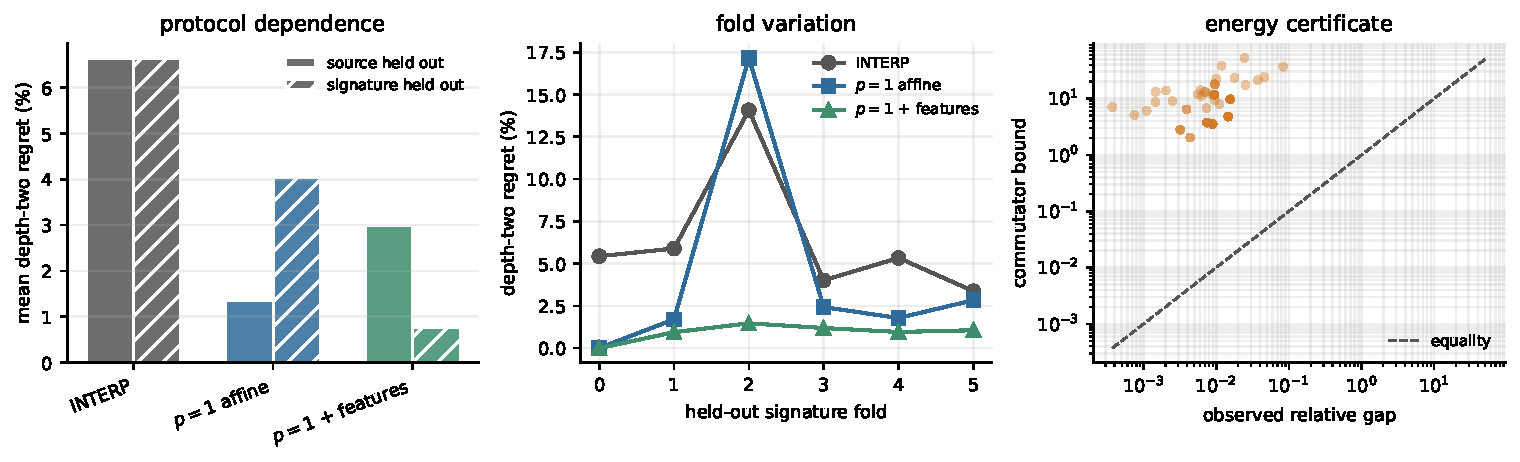
\includegraphics[width=\textwidth]{code/manuscript_assets/figures/depth_lifting.pdf}
\caption{\label{fig:depth}Depth-transfer evidence.  Left: mean depth-two regret
under two nonoverlapping evaluations.  Center: foldwise regret under the
collision-free feature-signature protocol.  Right: observed relative energy
gap and the bound in Theorem~\ref{thm:energy}; all points lie above the equality
line because the ordinate is the certificate.}
\end{figure}

The experiment does not establish optimal depth-two schedules, performance on
weighted graphs, or transfer to graphs outside the six Gset topologies.  It
does establish a reproducible distinction between interpolation, schedule-only
lifting, and graph-conditioned lifting under a split that prohibits identical
feature signatures across training and test data.

\section{Reproducibility}

The package stores source addresses, byte hashes, topology hashes, fold
assignments, hyperparameters, theorem checks, and all plotted values.  A single
command fetches the graph files, recomputes both protocols, regenerates the
tables and figures, and compares the result with the locked record after
excluding wall-clock fields.  Tests independently check topology
deduplication, fold disjointness, the affine construction, and all 144 energy
certificates.

\bibliographystyle{plainnat}
\bibliography{code/manuscript_assets/references}

\end{document}
